\section{Nixtla NeuralForecast}
{{\footnotesize
\begin{description}[labelwidth=5em, labelsep=1em, leftmargin=*, align=left, itemsep=0.3em, parsep=0em]
  \item[date:] 2022-04-01
  \item[last\_updated:] 2025-06
  \item[expired:] unkown
  \item[valid:] yes
  \item[url:] \href{https://github.com/Nixtla/neuralforecast}{https://github.com/Nixtla/neuralforecast}
  \item[domain:] Time-series forecasting; General ML
  \item[focus:] High-performance neural forecasting library with >30 models
  \item[keywords:]
    - time-series
    - neural forecasting
    - NBEATS, NHITS, TFT
    - probabilistic forecasting
    - usability
  \item[task\_types:]
    - Time-series forecasting
  \item[ai\_capability\_measured:]
    - Forecast accuracy
    - interpretability
    - speed
  \item[metrics:]
    - RMSE
    - MAPE
    - CRPS
  \item[models:]
    - NBEATS
    - NHITS
    - TFT
    - DeepAR
  \item[ml\_motif:]
    - Time-series
  \item[type:] Platform
  \item[ml\_task:] Forecasting
  \item[notes:] AutoModel supports hyperparameter tuning and distributed execution via Ray and Optuna. Fi­rst official NHITS implementation. :contentReference[oaicite:4]\{index=4\}
  \item[contact.name:] Kin G. Olivares (Nixtla)
  \item[contact.email:] unkown
  \item[results.name:] ChatGPT LLM
  \item[results.url:] \href{unkown}{unkown}
  \item[fair.reproducible:] Yes
  \item[fair.benchmark\_ready:] Yes
  \item[ratings.software.rating:] 0
  \item[ratings.software.reason:] Not analyzed.
  \item[ratings.specification.rating:] 9.0
  \item[ratings.specification.reason:] Targets high-throughput LLM inference via PagedAttention and memory-optimized serving; benchmarks cover many configs.
  \item[ratings.dataset.rating:] 7.0
  \item[ratings.dataset.reason:] Focuses on model configs and streaming input/output pipelines rather than classical datasets.
  \item[ratings.metrics.rating:] 9.0
  \item[ratings.metrics.reason:] Strong token/sec, memory usage, and TTFT metrics; comparative plots and logs included.
  \item[ratings.reference\_solution.rating:] 9.0
  \item[ratings.reference\_solution.reason:] Benchmarks reproducible via script with support for multiple models and hardware types.
  \item[ratings.documentation.rating:] 9.0
  \item[ratings.documentation.reason:] Excellent GitHub docs, CLI/API usage, and deployment walkthroughs.
  \item[id:] nixtla\_neuralforecast
  \item[Citations:] \cite{olivares2022library_neuralforecast}
  \item[Ratings:]
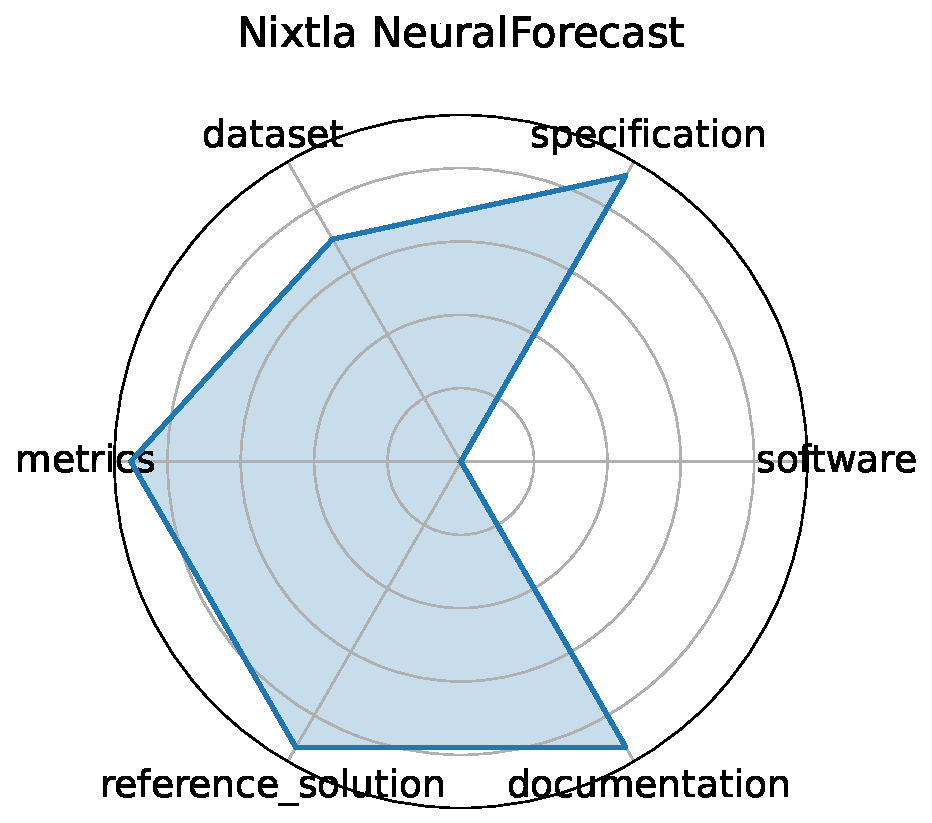
\includegraphics[width=0.2\textwidth]{nixtla_neuralforecast_radar.pdf}
\end{description}
}}
\clearpage